\section{Die Ableitung 1. Grades}
Die Ableitung 1. Grades beschreibt die Steigung an einem bestimmten Punkt der Funktion. In der Abbildung \ref{fig:00_steigung_an_punkt}
wird eine Funktion $f(x)$ (in grün) gegeben. Die Steigung $f'(x)$ an einem bestimmten Punkt $x$ ist rot markiert.
Die Ableitung selbst ist wiederum eine Funktion und kann über diverse Ableitungsregeln aufgrund der gegebenen Funktion
selbst gebildet werden.
\begin{figure}[h!]
    \begin{center}
        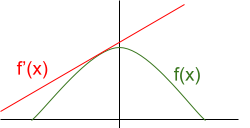
\includegraphics[width=0.4\linewidth]{../common/02_appendix/00_resources/00_derivation.png}
    \end{center}
    \caption{Steigung an einem bestimmten Punkt der Funktion $f(x)$}
    \label{fig:00_steigung_an_punkt}
\end{figure}

Die Ableitungsregeln, welche im Zuge der Erklärung des Lernprozesses eines neuronalen Netzwerks benötigt werden,
sind nachfolgend ersichtlich.
\begin{itemize}
    \item[Potenzregel] $f(x) = x^n \longrightarrow f'(x) = n \cdot x^{n-1}$\label{abl:potenzregel}
    \item[Kettenregel] $f(x) = u(v(x)) \longrightarrow f'(x) = u'(v(x)) \cdot v'(x)$\label{abl:kettenregel}
\end{itemize}
Es existieren viele weitere Ableitungsregeln, auf die hier nicht weiter eingegangen wird.
Die Schreibweise der Ableitung einer Funktion nach einer Variablen lautet $f'(x) = \frac{\delta f(x)}{\delta x}$.

\section{Die partielle Ableitung}
Ist der Input einer Funktion mehrdimensional, das heisst, die Funktion $f$ ist abhängig von mehreren Variablen, dann
kann die Ableitung jeweils lediglich nach einer Variablen gebildet werden. Die übrigen Variablen werden als konstant
angesehen. In dem Fall beschreibt die partielle Ableitung die Steigung an einem bestimmten Punkt der abgeleiteten
Dimension. Es sei als Beispiel die Funktion $f(x, z) = x^2 + z^2 + 10$ gegeben. Diese wird nun partiell nach $x$ sowie
nach $z$ abgeleitet.
\begin{align}
    f^x(x, z) = 2x\\
    f^z(x, z) = 2z
\end{align}
Die hierbei angewendete Ableitungsregel ist die Potenzregel, welche bereits im vorangegangenen Kapitel erwähnt wurde.

\section{Die Sigmoide}
Als Aktivierungsfunktion wird die Sigmoidfunktion benutzt. Diese wird heutzutage meist nicht mehr eingesetzt aufgrund
des schlechten Lernverhaltens in einigen Bereichen der Funktion. Die erwähnte Eigenschaft wird bei der Betrachtung
der Ableitung ersichtlich.
\begin{align}
    sig(t) = \frac{1}{1 + e^{-t}}
\end{align}
Geometrisch lässt sich die Funktion so interpretieren, dass eine gewisse Schwelle existiert, ab der die Funktion
den Eingabewert auf eine $1$ abbildet, in dem Jargon der Neuronen also \glqq feuert\grqq. Das Resultat lautet also
entweder $0$ oder $1$.
TODO: Bild

Für die weitere Verwendung ist nun vor allem die Ableitung der Sigmoide interessant, welche in den nachfolgenden
Zeilen behandelt wird. Zuerst wird der Bruch durch eine andere Schreibweise (Exponent $-1$) dargestellt.
\begin{align}
    sig(t) = (1 + e^{-t})^{-1} \longrightarrow y = 1 + e^{-t}, f(t) = y^{-1}
\end{align}
Es handelt sich also um eine äussere und innere Funktion, wobei nun die Ableitungsregel \ref{abl:kettenregel} angewendet wird.
Für die innere Ableitung wird nun noch die Regel für $e$ verwendet. TODO
\begin{align}
    \frac{\delta f(t)}{\delta t} = (-1) \cdot (y(t))^{-2}\\
    \frac{\delta y(t)}{\delta t} = (e^{-t}) \cdot (-1)
\end{align}
Nach der Kettenregel resultiert:
\begin{align}
    \frac{\delta sig(t)}{\delta t} = (-1) \cdot (1 + e^{-t})^{-2} \cdot (e^-t) \cdot (-1)\\
    \frac{\delta sig(t)}{\delta t} = \frac{e^{-t}}{(1 + e^{-t})^{2}}
\end{align}
Nun wird $\frac{1}{1 + e^{-t}}$ ausgeklammert.
\begin{align}
    \frac{\delta sig(t)}{\delta t} = \frac{1}{1 + e^{-t}} \cdot \frac{e^{-t}}{(1 + e^{-t})}
\end{align}
Beim Zähler wird 1 dazuaddiert und abgezogen, damit der Faktor umgeformt werden kann.
\begin{align}
    \frac{\delta sig(t)}{\delta t} = \frac{1}{1 + e^{-t}} \cdot \frac{e^{-t} + 1 - 1}{(1 + e^{-t})}\\
    \frac{\delta sig(t)}{\delta t} = \frac{1}{1 + e^{-t}} \cdot (\frac{1 + e^{-t}}{(1 + e^{-t})} - \frac{1}{1 + e^{-t}})
\end{align}
Es resultiert die Ableitung in bekannter Form \ref{eq:00_ableitung_sigmoide}
\begin{align}
    \frac{\delta sig(t)}{\delta t} = sig(t) \cdot (1 - sig(t))\label{eq:00_ableitung_sigmoide}
\end{align}

